\documentclass[11pt,a4paper]{article}

% Packages
\usepackage[utf8]{inputenc}
\usepackage[english]{babel}
\usepackage{caption}
\usepackage{listings}
\usepackage{adjustbox}
\usepackage{enumitem}
\usepackage{dsfont}
\usepackage{boldline}
\usepackage{amssymb, amsmath}
\usepackage[margin=1in]{geometry}
\usepackage{xcolor}
\usepackage{enumerate}
\usepackage{hyperref}
\usepackage{graphics, graphicx, float}
\usepackage{titlesec} %\titleformat

% Meta
\title{Introduction to Multivariate Data Analysis
	\\\medskip \large Final Project Report}
\author{José Antonio Álvarez Ocete - 917933752 \\ jocete@ucdavis.edu}
\date{ \today }

% Custom
\providecommand{\abs}[1]{\lvert#1\rvert}
\setlength\parindent{0pt}
\definecolor{Light}{gray}{.90}
\setlength{\parindent}{1.5em} %sangria

% Thicker lines in tables
\makeatletter
\newcommand{\thickhline}{%
	\noalign {\ifnum 0=`}\fi \hrule height 1pt
	\futurelet \reserved@a \@xhline
}
\makeatother

% Subsubsubsection (|paragraph)
\setcounter{tocdepth}{4}
\setcounter{secnumdepth}{4}

\begin{document}	
	
	\maketitle 
	\newpage
	\tableofcontents
	\newpage
	
	\section{Multiple Linear Regression}
	
	\subsection{Introduction}
	
	In this first section, we will conduct a multiple linear regression following question 1 of the 5th homework assignment. We will estimate the regression coefficients (betas) following different several methods seen during the lectures and we will provide an estimation for a new response.
	
	\subsection{Summary}
	
	For this first analysis, I've selected the Battery Failure dataset. In this example, we want to predict the cycles of life of a certain battery before it fails. We are provided the following variables: Charge rate (amps), discharge rate (amps), depth of discharge (\% of rated ampere-hours), temperature (ºC), and end of charge voltage (volts). These are the first three rows of data: 
	
	\begin{table}[H] \centering
		\begin{tabular}{|cccccc|}
			\hline
			\begin{tabular}[c]{@{}c@{}}Charge rate\\  (amps)\end{tabular} & \begin{tabular}[c]{@{}c@{}}Discharge Rate\\ (amps)\end{tabular} & \begin{tabular}[c]{@{}c@{}}Depth of \\ Discharge\\ (\% of rated\\ ampere-hours)\end{tabular} & \begin{tabular}[c]{@{}c@{}}Temperature\\ (ºC)\end{tabular} & \begin{tabular}[c]{@{}c@{}}End of\\ Charge\\ Voltage\\ (volts)\end{tabular} & \begin{tabular}[c]{@{}c@{}}Cicles to\\ failure\end{tabular} \\ \hline
			0.375                                                         & 3.13                                                            & 60.0                                                                                         & 40                                                         & 2.00                                                                        & 101                                                         \\
			1.000                                                         & 3.13                                                            & 76.8                                                                                         & 30                                                         & 1.99                                                                        & 141                                                         \\
			1.000                                                         & 3.13                                                            & 60.0                                                                                         & 20                                                         & 2.00                                                                        & 96                                                          \\ \hline
		\end{tabular}
	\end{table}
	
	\subsection{Analysis}
	
	\textbf{(1) Find the least square estimate beta hat} \\
	
	We obtain the least square estimate beta hat following out notes:
	
	$$ \hat{\vec{\beta}} = (Z^T \cdot Z)^{-1} \cdot Z^T \cdot \vec{Y} $$
	
	Obtaining:
	$$ \hat{\vec{\beta}} =
		\begin{pmatrix}
		-2937.7571 \\
		-33.7934   \\
		-0.1798   \\
		-1.7397    \\
		7.0627     \\
		1529.2897
		\end{pmatrix}
	$$
	
	\textbf{(2) Find the $R^2$ statistic} \\
	
	We use:
	
	$$ R^2 = \frac{||\hat{\vec{Y}} - \bar{Y} \cdot \vec{1_n}||^2}{||\vec{Y} - \bar{Y} \cdot \vec{1_n}||^2} $$
	
	Obtaining $R^2 = 0.4799$. \\
	
	\textbf{(3) Find sigma\_hat\_square and estimated Cov(beta square)} \\
	
	We use:
	
	$$ \hat{\sigma}^2 = \frac{1}{n-r-1} ||\hat{\vec{\epsilon}}||^2 $$
	
	and
	
	$$ \hat{Cov}(\hat{\vec{\beta}}) = \hat{\sigma}^2 (Z^T Z)^{-1} $$
	
	We obtain the following:
	
	$$ \hat{\sigma}^2 = 7138.186 $$	
	$$ \hat{Cov}(\hat{\vec{\beta}}) = 
	\begin{pmatrix}
	1.633e+07  & -2933.74 & 2980.4460  & -34.78143 & -991.73637 & -8.160e+06 \\
	-2.934e+03 & 1880.55  & 18.5503    & 17.34897  & 10.28445   & -1.764e+02 \\
	2.980e+03  & 18.55    & 193.4117   & -3.23257  & 0.34449    & -1.696e+03 \\
	-3.478e+01 & 17.35    & -3.2326    & 1.79944   & -0.08092   & -4.242e+01 \\
	-9.917e+02 & 10.28    & 0.3445     & -0.08092  & 3.89193    & 4.549e+02  \\
	-8.160e+06 & -176.39  & -1695.7845 & -42.42251 & 454.86652  & 4.081e+06 
	\end{pmatrix}
	$$ \\
	
	\textbf{(4) 95\% confidence interval for each $\beta_j$} \\
	
	We use one at a time confidence intervals for the betas:
	
	$$ \beta_j \in [ \hat{\beta_j} \pm \hat{\sigma} \cdot \sqrt{\omega_{jj}} \cdot t_{n-r-1}(\frac{\alpha}{2}) ] $$
	
	Obtaining:
	
	\begin{table}[H] \centering
		\begin{tabular}{l}
			$\beta_0 \in [ -11604 , 5729 ]$ \\
			$\beta_1 \in [ -126.8 , 59.22 ]$ \\
			$\beta_2 \in [ -30.01 , 29.65 ]$ \\
			$\beta_3 \in [ -4.617 , 1.137 ]$ \\
			$\beta_4 \in [ 2.831 , 11.29 ]$ \\
			$\beta_5 \in [ -2804 , 5862 ]$
		\end{tabular}
	\end{table}
	
	\textbf{(5) 95\% simultaneous confidence intervals for all betas based on the confidence region} \\
	
	Using the formula from the notes:
	
	$$ \beta_j \in [ \hat{\beta_j} \pm \hat{\sigma} \cdot \sqrt{\omega_{jj}} \cdot \sqrt{(r+1) \cdot F_{r+1,n-r-1}(\alpha)} ] $$
	
	We obtain:
	
	\begin{table}[H] \centering
		\begin{tabular}{l}
			$\beta_0 \in [ -19640 , 13764 ]$ \\
			$\beta_1 \in [ -213 , 145.5 ]$ \\
			$\beta_2 \in [ -57.67 , 57.31 ]$ \\
			$\beta_3 \in [ -7.285 , 3.805 ]$ \\
			$\beta_4 \in [ -1.092 , 15.22 ]$ \\
			$\beta_5 \in [ -6822 , 9880 ]$
		\end{tabular}
	\end{table}
	
	\textbf{(6) 95\% simultaneous confidence intervals for all betas based on the Bonferroni correction} \\
	
	We compute a final set of intervals for the ebtas using the Bonferroni correction:
	
	$$ \beta_j \in [ \hat{\beta_j} \pm \hat{\sigma} \cdot \sqrt{\omega_{jj}} \cdot t_{n-r-1}(\frac{\alpha}{2(r+1)}) ] $$
	
	We obtain:
	
	\begin{table}[H] \centering
		\begin{tabular}{l}
			$\beta_0 \in [ -15338 , 9462 ]$ \\
			$\beta_1 \in [ -166.9 , 99.29 ]$ \\
			$\beta_2 \in [ -42.86 , 42.5 ]$ \\
			$\beta_3 \in [ -5.856 , 2.377 ]$ \\
			$\beta_4 \in [ 1.009 , 13.12 ]$ \\
			$\beta_5 \in [ -4670 , 7729 ]$
		\end{tabular}
	\end{table}
	
	\textbf{(7) Test $H_0: \beta_1 = \beta_2 = 0 $ at significance level $\alpha = 0.05$} \\
	
	Using this matrix for the linear transformation:
	
	$$ C = 
	\begin{pmatrix}
		0 & 1 & 0 & 0 & 0 & 0 \\
		0 & 0 & 1 & 0 & 0 & 0 \\
		0 & 0 & 0 & 1 & 0 & 0 \\
		0 & 0 & 0 & 0 & 1 & 0 \\
		0 & 0 & 0 & 0 & 0 & 1
	\end{pmatrix}
	$$
	
	We can compute the F-test statistic:
	
	$$ \vec{\beta}^T_{(2)} \Omega_{22}^{-1} \vec{\beta}_{(2)} = 108296 $$
	
	And compare it to:
	
	$$ (r-q) \cdot \hat{\sigma}^2 \cdot F_{r-q,n-r-1}(\alpha) = 133445 $$
	
	Since $108296 < 133445$, we don't have sufficient evidence to assure that $\beta_1 = \beta_2 = 0$. \\
	
	\textbf{(8) 95\% confidence interval for the mean response given $\mathds{E}(Y_0) = \beta_0 + \sum_{i=1}^{5} \beta_i \cdot \bar{z}_i$, where $\bar{z}_i$ is the sample mean of $z_{i,j}$ for $i \in \{1, ..., n\}$} \\
	
	First, compute $\vec{z_0}$:
	
	$$ \vec{z_0} = 
	\begin{pmatrix}
		1.000  \\
		1.031  \\
		3.034  \\
		62.840 \\
		19.500 \\
		1.999 
	\end{pmatrix} 
	$$
	
	And now compute the confidence intervals for it's associated value using the formula in the class notes:
	
	$$ \vec{z_0}^T \vec{\beta} \in [\vec{z_0}^T \hat{\vec{\beta}} \pm \hat{\sigma} \cdot t_{n-r-1}(\frac{\alpha}{2}) \sqrt{\vec{z_0}^T (Z^T Z)^{-1} \vec{z_0}} ] $$
	
	Obtaining the following interval: $ \vec{z_0}^T \vec{\beta} \in [ 71.78 , 152.8 ] $ \\
	
	\textbf{(9) 95\% confidence interval for a new response $Y_0$ given $\vec{z_0}$} \\
	
	Using a similiar formula: 
	
	$$ \vec{z_0}^T \vec{\beta} \in [\vec{z_0}^T \hat{\vec{\beta}} \pm \hat{\sigma} \cdot t_{n-r-1}(\frac{\alpha}{2}) \sqrt{1 + \vec{z_0}^T (Z^T Z)^{-1} \vec{z_0}} ] $$
	
	And using that $Y_0 = \vec{z_0}^T \vec{\beta} + \epsilon_0$ we obtain:
	
	$$ Y_0 \in [ -73.38 , 298 ] $$
	
	A substantialy bigger interval than the over in \textbf{(8)}, which makes sense since we are including the error now.
	
	\section{Principal Component Analysis}
	
	\subsection{Introduction}
	
	For the second analysis we will conduct Principal Component Analysis on our dataset. Ourmain objectives will be to analyze the explained variance against the numbers of principal components in order to reduce the dimensionality of our dataset, as well as study how standarizing the data would affect these parameters.
	
	\subsection{Summary}
	
	In order to achieve those objetives we need to select a dataset relatively hihg dimensionality, at least compare to the rest of the datasets in the book, that will also yield different results upon standarizing the data. In order to fullfill this criteria I selected the Breakfast Cereal dataset. \\
	
	We this dataset we aim to distinguish cereals from three different manufacturers: General Mills (G), Kellogg (K), and Quaker (Q); by looking at 8 variates: Calories, Protein, Fat, Sodium, Fiber, Carbohydrates, Sugar, and Potassium. These are the first 3 rows of each manufacturer:
	
	\begin{table}[H] \centering
		\begin{tabular}{|l|llllllll|}
			\hline
			\multicolumn{1}{|c|}{Manufacturer} & \multicolumn{1}{c}{Calories} & Protein & Fat & Sodium & Fiber & Carbohydrates & Sugar & Potassium \\ \hline
			G                                  & 110                          & 2       & 2   & 180    & 1.5   & 10.5          & 10    & 1         \\
			G                                  & 110                          & 6       & 2   & 290    & 2.0   & 17.0          & 1     & 1         \\
			G                                  & 110                          & 1       & 1   & 180    & 0.0   & 12.0          & 13    & 55        \\
			K                                  & 70                           & 4       & 1   & 260    & 9.0   & 7.0           & 5     & 320       \\
			K                                  & 110                          & 2       & 0   & 125    & 1.0   & 11.0          & 14    & 30        \\
			K                                  & 100                          & 2       & 0   & 290    & 1.0   & 21.0          & 2     & 35        \\
			Q                                  & 120                          & 1       & 2   & 220    & 0.0   & 12.0          & 12    & 35        \\
			Q                                  & 120                          & 1       & 2   & 220    & 1.0   & 12.0          & 11    & 45        \\
			Q                                  & 100                          & 4       & 2   & 150    & 2.0   & 12.0          & 6     & 95        \\ \hline
		\end{tabular}
	\end{table}

	Although our data is quite unbalanced class-wise, this doesn't affect our PCA analysis.
	
	\subsection{Analysis}
	
	We start by computing basic stats of our data:
	
	
	$$ \bar{\vec{x}} = 
	\begin{pmatrix}
		107.9070 \\
		2.4651   \\
		0.9767   \\
		180.4651 \\
		1.7140   \\
		10.2093  \\
		7.6047   \\
		84.4186 
	\end{pmatrix}
	$$
	
	$$ S = 
	\begin{pmatrix}
		359.80 & 0.76  & 5.90  & 505.76  & -0.66  & 11.40  & 49.87  & 177  \\
		0.76   & 1.49  & 0.20  & 9.06    & 1.13   & 0.47   & -2.22  & 40   \\
		5.90   & 0.20  & 0.64  & 0.61    & 0.24   & -1.16  & 0.68   & 17   \\
		505.76 & 9.06  & 0.61  & 6274.78 & 6.18   & 182.28 & -17.55 & 599  \\
		-0.66  & 1.13  & 0.24  & 6.18    & 3.24   & 0.92   & -0.28  & 110  \\
		11.40  & 0.47  & -1.16 & 182.28  & 0.92   & 20.88  & -5.30  & 20   \\
		49.87  & -2.22 & 0.68  & -17.55  & -0.28  & -5.30  & 20.58  & 24   \\
		177.33 & 40.40 & 16.53 & 599.09  & 110.48 & 19.53  & 24.41  & 4370                 
	\end{pmatrix} 
	$$ 
	
	In order to run PCA we compute the spectral decomposition of $S$:
	
	$ S = V \Lambda V^T$
	
	Where:
	
	$$ V = 
	\begin{pmatrix}
		-0.087 & 0.008  & 0.982  & 0.104  & 0.124  & 0.020  & -0.035 & 0.000  \\
		-0.003 & 0.009  & -0.005 & 0.079  & 0.197  & -0.930 & 0.276  & 0.117  \\
		-0.001 & 0.004  & 0.017  & -0.042 & 0.096  & 0.184  & 0.802  & -0.558 \\
		-0.957 & -0.279 & -0.079 & -0.034 & 0.004  & -0.001 & -0.001 & -0.001 \\
		-0.006 & 0.025  & -0.015 & 0.035  & -0.021 & -0.255 & -0.508 & -0.821 \\
		-0.028 & -0.008 & -0.016 & 0.824  & -0.555 & -0.017 & 0.106  & -0.011 \\
		0.001  & 0.007  & 0.165  & -0.547 & -0.793 & -0.187 & 0.100  & -0.009 \\
		-0.277 & 0.960  & -0.032 & -0.002 & 0.000  & 0.015  & 0.008  & 0.022 
	\end{pmatrix} 
	$$ 
	
	$$ \Lambda = 
	\begin{pmatrix}
		6499.572 & 0        & 0       & 0      & 0     & 0     & 0     & 0     \\
		0        & 4201.334 & 0       & 0      & 0     & 0     & 0     & 0     \\
		0        & 0        & 321.556 & 0      & 0     & 0     & 0     & 0     \\
		0        & 0        & 0       & 18.435 & 0     & 0     & 0     & 0     \\
		0        & 0        & 0       & 0      & 9.642 & 0     & 0     & 0     \\
		0        & 0        & 0       & 0      & 0     & 0.677 & 0     & 0     \\
		0        & 0        & 0       & 0      & 0     & 0     & 0.397 & 0     \\
		0        & 0        & 0       & 0      & 0     & 0     & 0     & 0.287
	\end{pmatrix} 
	$$ 
	
	As we can see, our first two eigen values are way larger than the rest. By looking at the loading in $V$ we can see how these first two principal components are essetially the first and sixth variable respectively. Selecting the first two principal components from this analysis isn't much different from selecting those two variables. As we will see, they explain the variance pretty well, but that's only because the data is not standarized and the scale makes a huge different. Using the following result:
	
	$$ \sum_{i=1}^{n} \lambda_i = \sum_{i=1}^{n} \sigma_i^2 $$
	
	We can compute the ratio of explained variance by the first two principal components:
	
	$$ Explained \ variance = \frac{\lambda_1 + \lambda_2}{\sum_{i=1}^{n} \lambda_i} = 0.968 $$
	
	Let's study now how our data behaves if it's standarized. we obtain the spectral decomposition of the correlation matrix, which is the covariance matrix of the standarized data, and obtain the following:
	
	 $$ V_z = 
	 \begin{pmatrix}
		 -0.161 & -0.540 & -0.370 & 0.13  & 0.45  & -0.040 & 0.562  & -0.069 \\
		-0.454 & 0.233  & 0.093  & 0.41  & 0.57  & 0.323  & -0.375 & 0.013  \\
		-0.261 & -0.409 & 0.182  & 0.58  & -0.37 & -0.453 & -0.221 & -0.071 \\
		-0.167 & 0.012  & -0.640 & 0.18  & -0.50 & 0.518  & -0.063 & -0.053 \\
		-0.561 & 0.096  & 0.145  & -0.38 & -0.12 & -0.041 & 0.123  & -0.694 \\
		-0.114 & 0.284  & -0.615 & -0.15 & 0.16  & -0.624 & -0.298 & 0.043  \\
		0.032  & -0.630 & -0.040 & -0.44 & 0.12  & 0.170  & -0.602 & -0.016 \\
		-0.586 & -0.034 & 0.110  & -0.29 & -0.16 & -0.015 & 0.159  & 0.710 
	 \end{pmatrix} 
	 $$ 
	 
	 $$ \Lambda_z = 
	 \begin{pmatrix}
		2.49  & 0        & 0       & 0      & 0     & 0     & 0     & 0     \\
		0        & 1.89 & 0       & 0      & 0     & 0     & 0     & 0     \\
		0        & 0        & 1.63 & 0      & 0     & 0     & 0     & 0     \\
		0        & 0        & 0       & 0.91 & 0     & 0     & 0     & 0     \\
		0        & 0        & 0       & 0      & 0.50 & 0     & 0     & 0     \\
		0        & 0        & 0       & 0      & 0     &0.39 & 0     & 0     \\
		0        & 0        & 0       & 0      & 0     & 0     & 0.13 & 0     \\
		0        & 0        & 0       & 0      & 0     & 0     & 0     & 0.05
	 \end{pmatrix} 
	 $$ 
	 
	 As we can see, the eigen values are now much more closer to each other, and the loadings are way more balanced. 
	 
	 \begin{figure}[H] 
	 	\centering
	 	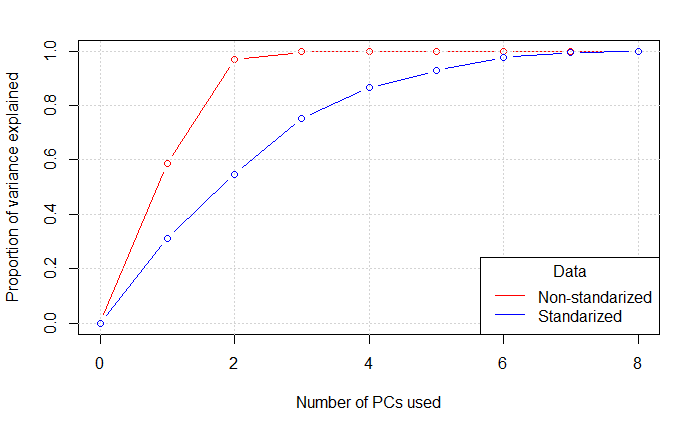
\includegraphics[scale=.9]{./pics/PCA1}
	 	\caption{Portion of explained variance comparison} \label{variance-label}
	 \end{figure}
	
	In \ref{variance-label} we see how the growth of the proportion of variance explained with the standarized data is much more progresive. As we hypothesized before, with the non-standarized analysis we were using certain variables just because their variance was bigger. Now ous principal components use information for more variates, gaining more information of the whole dataset with fewer of them. \\
	
	For the rest of the anaylsis let's stick to the first two principal components. Let's transform our data using them and plot it:
	
	\begin{figure}[H] 
		\centering
		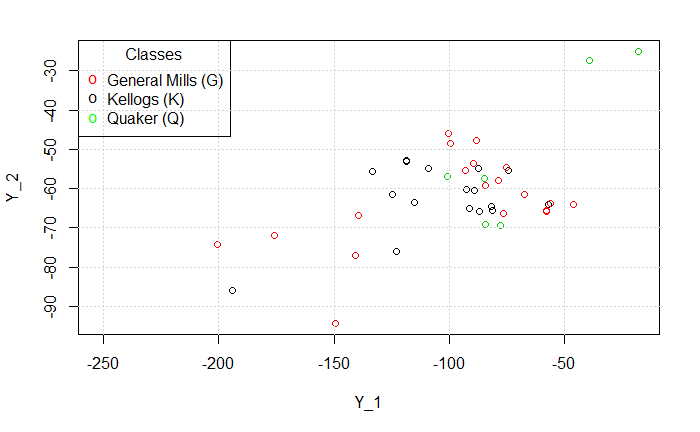
\includegraphics[scale=.9]{./pics/PCA2}
		\caption{Portion of explained variance comparison} \label{Y-dataset-label}
	\end{figure}
	
	We can see how our classes are not clearly separated, but that's not the main point of PCA. However the points are fairly spread out. After all, we are only explaining $55\%$ of our variance with the first two principal components. Finally, let's study how each variate contributes to these PCs. In order to do this we look at the loading of these PCs: studying only the first two columns of $V_z$ (our first two PCs), and plotting their rows we can see the variate contributions. \\
	
	In \ref{contributions-label} see each variate contribution as a colored vector. The bigger the vector, the greater the contribution, while the direction shows towards which principal component it contributes and wether it's a direct or inverse contribution. \\
	
	We can see how the variates $X_4$ and $X_6$ contribute the least to the first two principal components. On one hand, $X_1$ and $X_7$ contribute mostly to the first PC, $Y_1$. On the other hand, $X_5$ and $X_8$ contribute mostly to $Y_2$. Finally, $X_2$ and $X_3$ contribute to greatly to both PCs but in very different ways.
	
	\begin{figure}[H] 
		\centering
		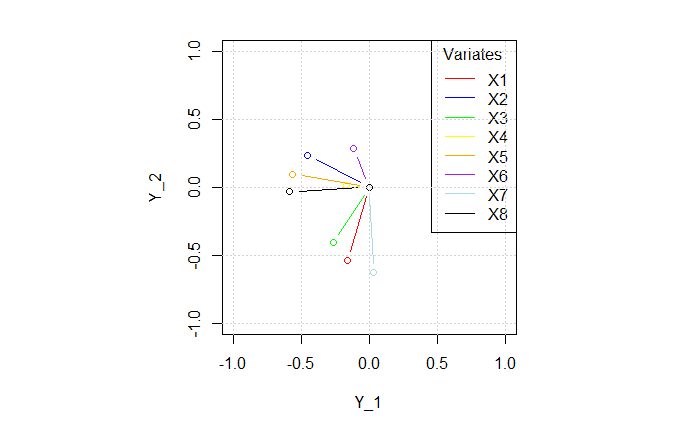
\includegraphics[scale=.9]{./pics/PCA3}
		\caption{Portion of explained variance comparison} \label{contributions-label}
	\end{figure}

	
	
	\section{Two-Sample test and Linear Discriminant Analysis}
	
	\subsection{Introduction}
	
	For this final analysis we will conduct Linear Discriminant Analysis. That is, given enough data about tagged as two different classes, classify a new reponse into one of this classes. In order to do that we first need to conduct a two sample test to make sure that our populations are actually different.
	
	\subsection{Summary}
	
	The dataset selection for this example was a little trickier since I wanted to display nice graphs about the data. In order to achieve this the more convinient way was to pick up a two-variate dataset with a nice visual separation between its classes. We will see why in the analysis. \\
	
	The dataset selected was the Anaconda one. It has two variates: Snout vent length and weight. The class we want to predict is the snake gender: either male (M) or female (F). These are the first 5 rows of our dataset from each class:
	
	\begin{table}[H] \centering
		\begin{tabular}{|ccc|ccc|}
			\hline
			Snout Vent Length & Weight & Gender & Snout Vent Length & Weight & Gender \\ \hline
			271.0             & 18.50  & F      & 176.7             & 3.00   & M      \\
			477.0             & 82.50  & F      & 259.5             & 9.75   & M      \\
			306.3             & 23.40  & F      & 258.0             & 10.07  & M      \\
			365.3             & 33.50  & F      & 229.8             & 7.50   & M      \\
			466.0             & 69.00  & F      & 233.0             & 6.25   & M      \\
			440.7             & 54.00  & F      & 237.5             & 9.85   & M      \\ \hline
		\end{tabular}
	\end{table}
	
	Our dataset is completely balanced, having the same number of males than females.
	
	\subsection{Analysis}
	
	As stated in the introduction we start by conduction a two sample test with the null hypothesis $H_0: \mu_1 = \mu_2$. We start by extracting the basic stats from the data and computing the Hotelling's $T^2$ statistic:
	
	$$ \bar{\vec{x_1}} = 
	\begin{pmatrix}
	348.28  \\         
	37.26
	\end{pmatrix} 
	, \bar{\vec{x_2}} = 
	\begin{pmatrix}
	228.75  \\         
	7.29
	\end{pmatrix} 
	$$
	
	$$ S_{pooled} = 
	\begin{pmatrix}
		\multicolumn{1}{c}{2606.4} & \multicolumn{1}{c}{667.9} \\
		667.9                      & 204.2                    
	\end{pmatrix} 
	$$ 
	
	$$ T^2 = (\bar{\vec{x_1}} - \bar{\vec{x_2}})^T ((\frac{1}{n_1} + \frac{1}{n_2}) S_{pooled})^{-1} (\bar{\vec{x_1}} - \bar{\vec{x_2}}) = 76.92 $$ 
	
	We compare this value to:
	
	$$ F = \frac{(n_1 + n_2 - 2)p}{n_1+n_2-1-p} \cdot F_{p, n_1+n_2-1-p}(\alpha) = 6.463 $$
	
	Since $76.92 > 6.463$, we reject $H_0$, concluding that both population are, indeed, different. We can now procede with linear discrimination analysis. For a given new response $\vec{x_0}$ we will classify it in the first population if and only if:
	
	$$ (\bar{\vec{x_1}} - \bar{\vec{x_2}})^T \cdot S_{pooled}^{-1} \cdot (\vec{x_0} - \frac{1}{2}(\bar{\vec{x_1}} - \bar{\vec{x_2}})) \ge 0 $$
	
	That is, if and only if:
	
	$$ 0.05095 - 0.01986 \cdot (\vec{x_0} - \begin{pmatrix}
	288.5 \\
	22.28
	\end{pmatrix} ) \ge 0 $$
	
	In order to meassure how good this classifier is we use two methods:
	
	\begin{itemize}
		\item The Apparent Error Rate (AER): Try to predict every single sample by training the model with every point in the dataset (including the one we will predict), and the use it for the prediction.
		\item The Expected Actual Error Rate (EAER): Using the same tachnique but exclude the point that we will predict from the train set.
	\end{itemize}

	In this case we obtain the same value for both measures: a $0.08929 = \frac{5}{56}$ error rate, missing 5 samples. Finally, let's plot our populations and their respective mean-centered mahalanobis-distance elipses to gain a geometry perspective of what is going on here:
	
	\begin{figure}[H] 
		\centering
		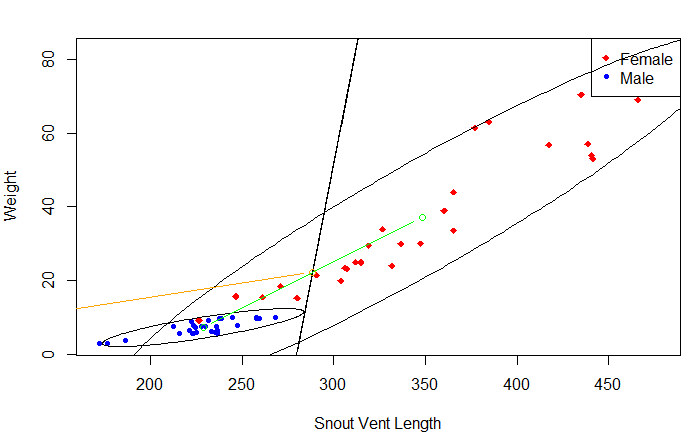
\includegraphics[scale=.9]{./pics/LDA}
		\caption{Anaconda dataset partition} \label{anaconda-label}
	\end{figure}
	
	In this figure we can see the two different classes in red (female) and blue (male). We have also plotted each population mean-centered elipse and a green line joining their centers. We can rewrite our test using the following: $\vec{x_0}$ will be classified as Female (class 1) if and only if:
	
	$$ \vec{\omega}^T \cdot \vec{\omega}_0 \ge 0 $$
	
	Where:
	
	$$ \vec{\omega} = (\bar{\vec{x_1}} - \bar{\vec{x_2}})^T \cdot S_{pooled}^{-1} $$
	$$ \vec{\omega}_0 = (\vec{x_0} - \frac{1}{2}(\bar{\vec{x_1}} - \bar{\vec{x_2}})) $$
	
	What we are computing here is the cosine of the angle between $\vec{\omega}$ and $\vec{\omega}_0$. If the absolute value of the angle is less than 90º, the cosine will be positive, so we are just studying this angel. In \ref{anaconda-label}, we plot $\vec{\omega}$ in orange, while $\vec{\omega}_0$ will be a vector from the middle point of the green segment to the given new responde $\vec{x_0}$. \\
	
	The easiest way to see this geometrically is to plot a perpendicular line to $\vec{\omega}$. This is the black line (although it doesn't seem perpendicular, this is because of the different scale in the axis). If the point is on the right side of the line, $\vec{\omega}_0$ and $\vec{\omega}$ will create an angle smaller than 90º, classifying $\vec{x_0}$ as Female, while if the point is on the left side of the line, $\vec{\omega}_0$ and $\vec{\omega}$ will create an angle greater than 90º, classifying $\vec{x_0}$ as Male.
	
\end{document}